\chapter{Herramientas y técnicas}
\lhead{\emph{Herramientas y técnicas}}

\begin{cabstract}
En el que se detalla el análisis de diferentes alternativas de aplicaciones, herramientas y técnicas para su uso en la construcción del sistema final y las decisiones finales tomadas.
\end{cabstract}

\section{Herramientas utilizadas para la creación del sistema}

\subsection{Lenguajes de programación}

Python se ha elegido como lenguaje principal de desarrollo. Es un lenguaje de programación interpretado de propósito general que prioriza la legibilidad del código y la rapidez de desarrollo, manteniendo estas propiedades en proyectos de cualquier escala. Este lenguaje soporta diferentes paradigmas de programación, entre ellos la orientación a objetos, programación imperativa y la programación funcional. Automatiza la gestión de memoria y utiliza un sistema de tipado dinámico rígido.

La gran cantidad de bibliotecas disponibles para el lenguaje y su facilidad de uso, así como el hecho de que la fundación Raspberry Pi propicie su uso en los equipos que produce constituyen ventajas competitivas sobre el resto de alternativas.

Junto a Python se han utilizado varios lenguajes de forma complementaria.

\begin{landscape}
\begin{table}[H]
\begin{tabular}{|p{1.4cm}|p{3.7cm}|p{3.5cm}|p{5cm}|p{7.5cm}|}
\hline
\textbf{Nombre} & \textbf{Características} & \textbf{Ventajas} & \textbf{Inconvenientes} & \textbf{Inclusión en el sistema}\\ \hline

\textbf{Python} & Orientación a objetos, portable & Portable, buen rendimiento & Necesidad de un intérprete & Se incluye en los componentes de alto nivel del sistema.\\ \hline

\textbf{C} & Imperativo, acceso a características de muy bajo nivel de forma sencilla & Muy eficiente e integrable en cualquier contexto & El desarrollo en el lenguaje suele ser más complejo que en otros lenguajes de más alto nivel & Se incluye en componentes que trabajan con entornos tediosos donde el rendimiento es crucial, o no se puede contar con un intérprete de Python. \\ \hline

\textbf{C}++ & Orientado a objetos & Gran rendimiento, acceso a todas las características de C & No es portable fácilmente en algunos casos & Se han creado los \textit{bindings} de MarcoPolo para este lenguaje, así como las herramientas \textbf{marcobootstrap}\\ \hline

\textbf{Java} & Orientado a objetos & Multiplataforma, popular y sencillo de utilizar & El rendimiento del lenguaje y su \textit{JVM} en el sistema son inferiores al de otras alternativas & Se utiliza en los paquetes \textit{software} que hacen uso de \textbf{Tomcat} y se ha creado un \textit{binding} de MarcoPolo para el lenguaje.\\ \hline

\textbf{Bash} & Lenguaje de comandos utilizado en sistemas UNIX & Interpretado, portable, sencillo de utilizar. & Es el lenguaje idóneo para una serie  concreta de aplicaciones, pero su propósito específico limita su uso más allá de dicho conjunto. & Utilizado en todos los \textit{scripts} de gestión de \textit{daemons} de systemv, y de arranque en \textbf{marcobootstrap}, así como herramienta de gestión en varias aplicaciones más.\\ \hline

\textbf{Perl} & Multiplataforma y multiparadigma & Portable, sencillo de utilizar, diseñado para la administración de sistemas & El uso de Perl como lenguaje de programación principal puede dificultar la realización de una serie de tareas clave. & Ninguna\\ \hline
\end{tabular}
\caption[Lenguajes de programación evaluados]{Lenguajes de programación evaluados para su utilización en el sistema y uso final}
\end{table}
\end{landscape}

\paragraph{Otros lenguajes\\}

Todas las interfaces web han sido programadas utilizando HTML, CSS y JavaScript en el lado del cliente. Dicha combinación evita la dependencia con cualquier herramienta no incluida por defecto en la totalidad de los navegadores mayoritarios (tales como Flash, ActiveX\dots).

\section{Herramientas utilizadas para la creación de \textit{software}}

\subsection{Twisted}

\textbf{Twisted} \footnote{\href{https://twistedmatrix.com/}{https://twistedmatrix.com/}} es un motor dirigido por eventos para la creación de aplicaciones basadas en red. Uno de los principales beneficios de la programación orientada a eventos es la capacidad del sistema de optimizar el tiempo de CPU y evitar cambios de contexto, pues todo el código se ejecuta en un único hilo. \textbf{Twisted} se basa en el patrón de diseño \textbf{reactor} (ver \ref{teoria:reactor}), que se basa en la gestión de diferentes eventos, su demultiplexación y el envío a los manejadores apropiados de forma síncrona (ver \ref{teoria:eventdriven}).

\textbf{Twisted} permite crear de forma sencilla sockets asíncronos a bajo nivel en los protocolos UDP y TCP y aplicaciones que utilizan protocolos bien definidos, como HTTP o DNS. Es capaz de trabajar con protocolos como \textbf{multicast} o \textbf{TLS} e integra funcionalidades para el desarrollo dirigido por pruebas (\textit{test-driven development}).

\textbf{Twisted} se ha utilizado para la creación de la herramienta de descubrimiento de servicios \textbf{MarcoPolo} (ver \ref{marcopolo}) y parte de la herramienta \textbf{PoloUsers} (ver \ref{polousers}).

Esta herramienta es elegida sobre otras alternativas analizadas:

\begin{itemize}
\item asyncore\footnote{\href{https://docs.python.org/3.5/library/asyncore.html}{https://docs.python.org/3.5/library/asyncore.html}} se plantea como la primera alternativa y es descartado por la incapacidad de desarrollar un prototipo funcional.
\item El bucle de eventos \texttt{io\_loop} de Tornado\footnote{\href{http://www.tornadoweb.org/en/stable/ioloop.html}{http://www.tornadoweb.org/en/stable/ioloop.html}}, si bien no diseñado específicamente para este propósito se considera como una alternativa viable. Sin embargo, la carencia de las facilidades para manejo de una aplicación en red (si bien Tornado es un servidor web, no está diseñado para implementar operaciones a bajo nivel, apoyándose siempre en protocolos como HTTP o WebSocket) hace que no sea una alternativa viable.
\end{itemize}

\textbf{Twisted} es elegido por la gran cantidad de protocolos que soporta y la posibilidad de manipular la pila de protocolos desde el nivel de red.

\subsection{Tornado}

\textbf{Tornado} es un \textit{framework} web y una biblioteca para aplicaciones en red que utiliza mecanismos de entrada/salida asíncrona, permitiendo crear herramientas como \textbf{WebSockets} de forma sencilla y escalable. Todo el código, a menos que explícitamente se indique lo contrario, se ejecuta en un único hilo.

\textbf{Tornado} se utiliza en todas las interfaces web creadas, en ocasiones en conjunción con \textbf{Django} y se integra con \textbf{MarcoPolo} a través del \textit{binding} para Python.

Si bien existen alternativas como node.js que siguen paradigmas similares, se decide utilizar Tornado debido a su implementación en Python, lenguaje conocido previamente, de alto rendimiento y fácil de utilizar para tareas que dependan altamente de la interacción con el sistema operativo y aplicaciones locales. Se descarta también utilizar herramientas web escritos en Python que por su arquitectura (basada en múltiples procesos o hilos) consuman más recursos, como el \textit{framework} Django.

\subsection{Websockets}

El protocolo WebSocket \cite{rfc6455} posibilita el establecimiento de un canal bidireccional en una arquitectura cliente-servidor sobre el protocolo HTTP/HTTPS evitando el uso de peticiones asíncronas (\texttt{XmlHttpRequest}, \texttt{<iframe>}) y \textit{polling}.

La mayoría de las interfaces web creadas utilizan este tipo de comunicación para obtener información desde los diferentes nodos del sistema, optimizando la comunicación al reducirse el intercambio de datos al momento en el que estos son necesarios (al contrario de otras estrategias) y posibilitando la difusión de eventos en directo, en contraste con estrategias como el \textit{polling}.

\section{Seguridad}

\subsection{OpenSSL}

\textbf{OpenSSL}\footnote{\href{https://www.openssl.org/}{https://www.openssl.org/}} es la implementación de código abierto más popular de los protocolos SSL y TSL. En el sistema se utiliza de forma intensiva para garantizar la confidencialidad de las transmisiones entre partes así como para verificar la identidad en ambos lados de un canal de comunicación. La biblioteca proporciona \textit{bindings} a C, C++, Java y Python, por lo que su integración en cualquiera de las herramientas creadas ha sido trivial. 

\subsection{Hadoop}

Hadoop\footnote{\href{https://hadoop.apache.org/}{https://hadoop.apache.org/}} es una herramienta diseñada para el procesamiento de grandes cantidades de datos de forma distribuida y el almacenamiento distribuido de información. La biblioteca ofrece además un gran nivel de fiabilidad mediante una serie de mecanismos de detección y gestión de errores. Es una de las herramientas de gestión de datos más popular actualmente.

En una de las iteraciones del ciclo de desarrollo se instaló parcialmente una instancia de Hadoop en el sistema. Sin embargo se descartó su continuación al priorizar una serie de tareas de mayor importancia. No obstante, se contempla como línea de trabajo futuro, y teóricamente es integrable con \textbf{MarcoPolo} a través de \texttt{marcomanager}.

No se ha realizado evaluación de otras alternativas para el proceso de grandes cantidades de datos, como \textbf{Apache Spark} \footnote{\href{https://spark.apache.org/}{https://spark.apache.org/}}.

\section{Aplicaciones distribuidas}

\subsection{\textit{Message Passing Interface}}

La necesidad de una herramienta de comunicación independiente de la plataforma derivó en la especificación del estándar MPI \cite{MPISpec}, un conjunto de interfaces para la creación de aplicaciones paralelas mediante la gestión de las operaciones de entrada-salida, definición de tipos de datos, grupos de proceso, creación y gestión de procesos, interfaces externas, etcétera. La especificación se define independientemente del lenguaje, si bien incluye implementaciones en C, C++ y Fortran, así como mecanismos para ser integrado con Python, entre muchos otros lenguajes.

MPI se ha convertido con el paso de los años en la interfaz de referencia para la creación de aplicaciones distribuidas, contando con varias implementaciones como \textbf{MPICH}\footnote{\href{https://www.mpich.org/}{https://www.mpich.org/}} (la implementación original) u \textbf{OpenMPI}\footnote{\href{http://www.open-mpi.org/}{http://www.open-mpi.org/}} (presente en la mayoría de supercomputadores), de tipo libre, o implementaciones propietarias tales como IBM MPI, Intel MPI, Cray MPI o Microsoft MPI.

MPI es utilizado en el sistema como herramienta de desarrollo de aplicaciones distribuidas, utilizando \textbf{MarcoPolo} para simplificar el proceso de descubrimiento de nodos (ver \ref{marcodiscover}). Además se han creado herramientas accesorias para facilitar varias tareas generalmente necesarias durante el desarrollo con la biblioteca (ver \ref{marcoinstallkey}).

La popularidad de MPI sobre otras herramientas similares como \textbf{PVM} (\textit{Parallel Virtual Machine}) \footnote{\href{http://www.csm.ornl.gov/pvm/}{http://www.csm.ornl.gov/pvm/}} hace que la cantidad de soporte para las placas Raspberry sea mayor. Esta circunstancia junto al hecho de que MPI es utilizado en la asignatura Arquitectura de Computadores (y por tanto se cuenta con experiencia de uso, y el desarrollo del sistema relativo a este tipo de aplicaciones podría utilizarse en la asignatura) hace que MPI sea la alternativa elegida sin evaluación previa.

\vspace{1cm}

Durante la etapa de desarrollo del sistema se han utilizado las dos vertientes libres más populares, \textbf{MPICH} y \textbf{OpenMPI}, siendo esta última la que se incluye en la versión final.

\subsubsection{\textit{Raspberry Pi Planet Simulator Cluster}}

Este proyecto implementa un simulador del clima terráqueo, permitiendo alterar diferentes características del mismo y analizar el resultado. Se implementa sobre MPI y está programado en el lenguaje \textbf{Fortran}\footnote{\href{http://econnexus.org/projects/the-distributed-arctic-sea-ice-model/raspberry-pi-planet-simulator-cluster/}{http://econnexus.org/projects/the-distributed-arctic-sea-ice-model/raspberry-pi-planet-simulator-cluster/}}.

\begin{figure}[H]
	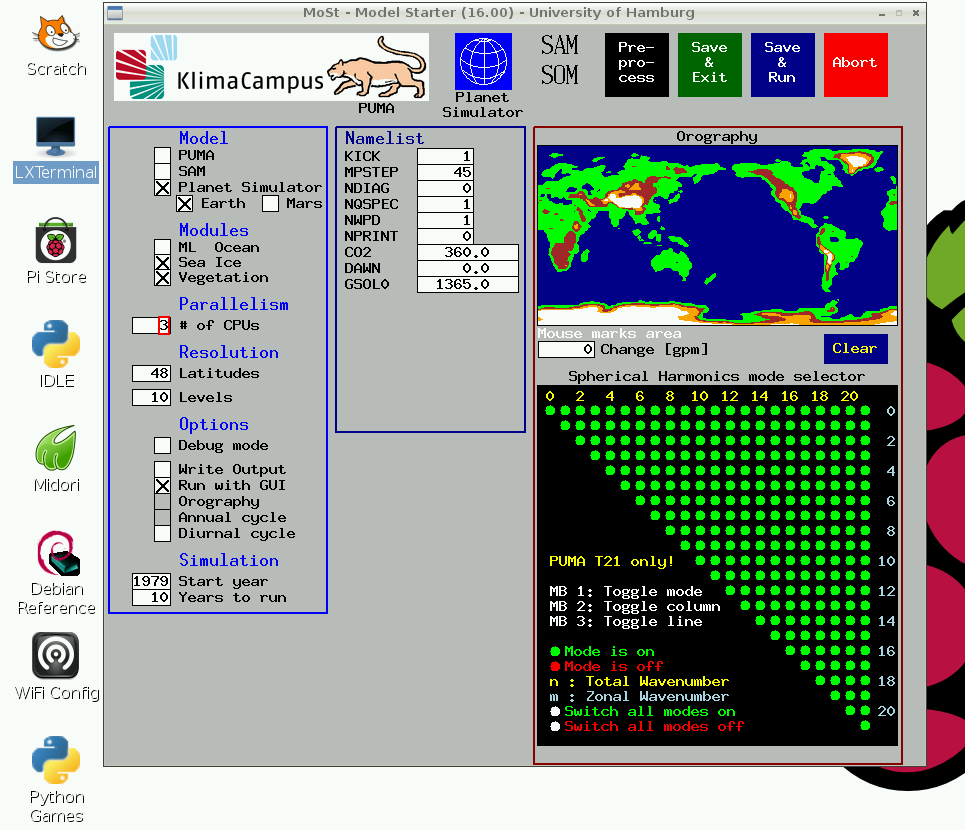
\includegraphics[height=12em]{Chapters/Chapter3/Figures/plasim-main}
	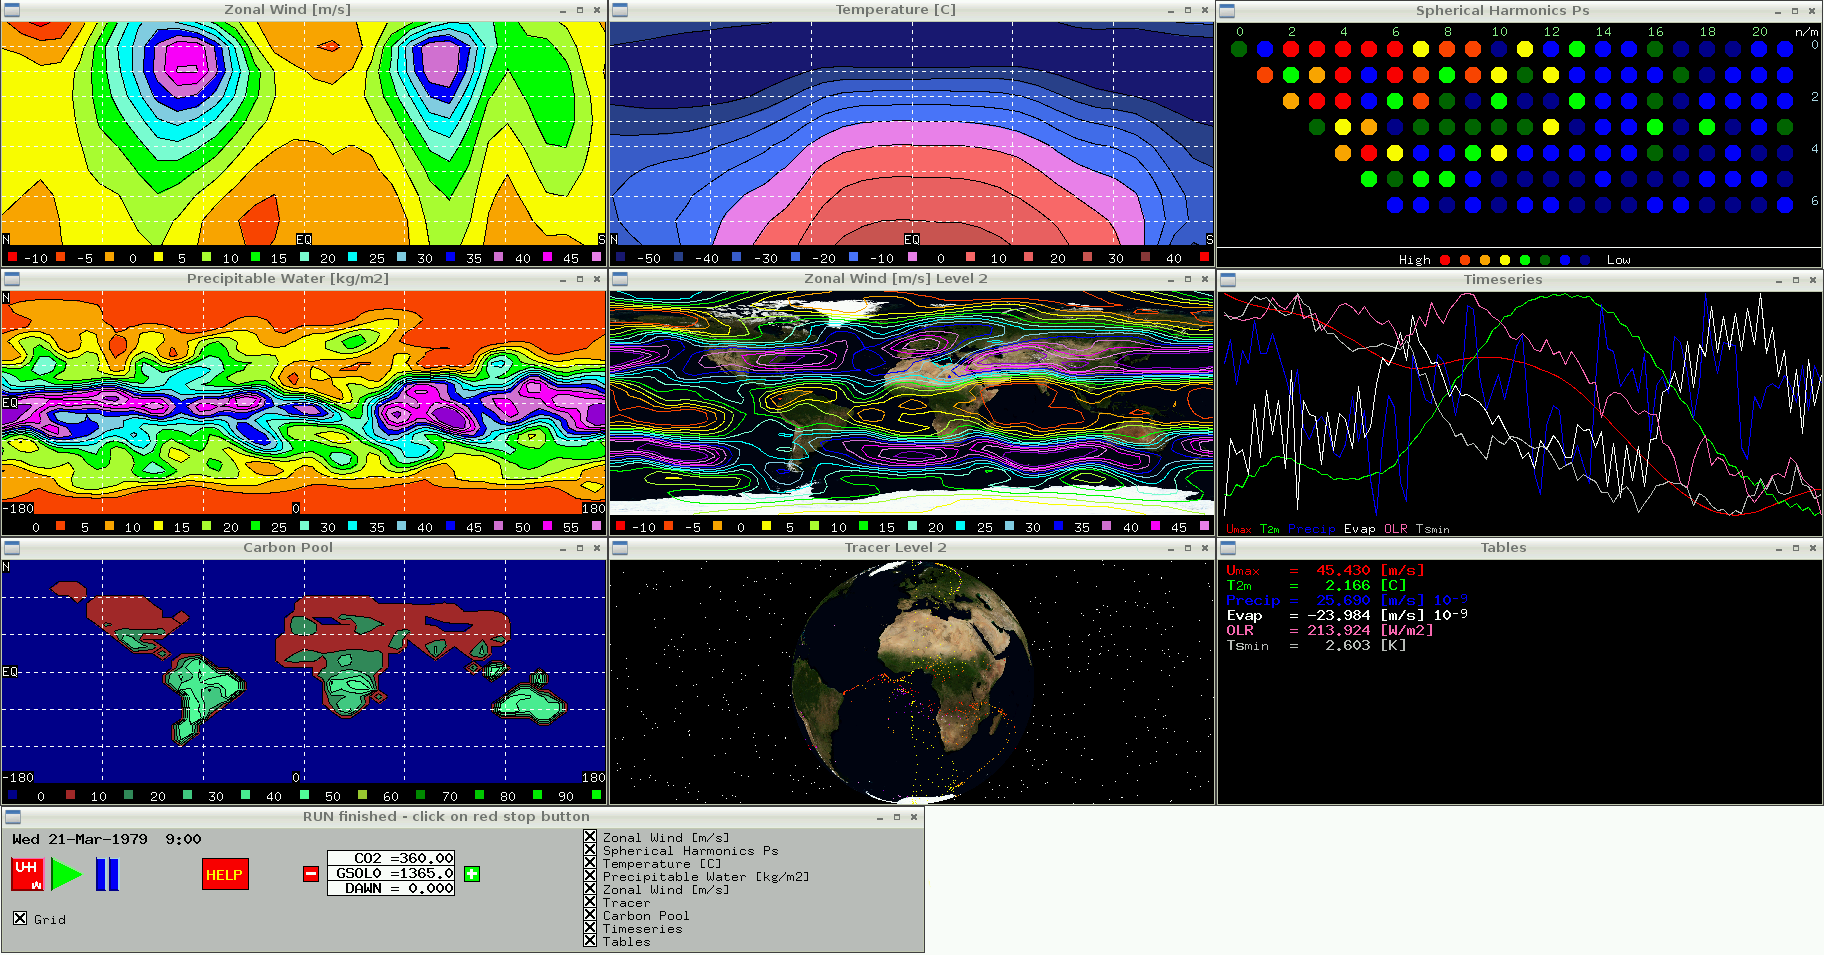
\includegraphics[height=12em]{Chapters/Chapter3/Figures/plasim-results}
	\label{fig:plasim}
	\caption[Interfaz de la aplicación \textit{Planet Simulator}]{Interfaz de control del \textit{Planet Simulator} y vista de ejecución de una simulación}
\end{figure}

Este proyecto ha sido evaluado con el objetivo de integrarlo en el sistema. Sin embargo, el programa depende considerablemente de la interfaz gráfica del mismo, inaccesible desde cualquiera de los nodos del sistema. A fin de solventar este problema se plantea el uso de un equipo de escritorio que cree los ficheros de configuración y los distribuya entre los nodos. Esta posibilidad se debe descartar finalmente, dado que el simulador realiza la compilación del programa con los parámetros fijados en la interfaz gráfica. Dado que los binarios creados para la arquitectura de un equipo de escritorio (x86, x86-64) son incompatibles con el \textit{hardware} de los nodos (arquitectura ARM) y hay tareas con mayor prioridad, se descarta esta tarea de forma indefinida, siendo finalmente no incluido en la versión final del sistema.

\subsection{Tomcat}

Las prácticas de la asignatura Sistemas Distribuidos se realizan sobre el contenedor de servicios Tomcat y el \textit{framework} Glassfish \footnote{\href{https://glassfish.java.net/}{https://glassfish.java.net/}} para la creación de APIs \textbf{REST}. Por ello el sistema ofrece instancias de Tomcat a todos los usuarios sin que estos deban realizar ningún tipo de configuración. Además, se habilita el uso de Tomcat en herramientas como \textbf{deployer} para facilitar el desarrollo de las prácticas.

Se plantea el análisis de alternativas para la creación de APIs \textbf{REST} como el \textit{framework} \textbf{Flask}.

\section{Herramientas de virtualización}

\subsection{QEMU}

QEMU\footnote{\href{http://qemu.org}{http://qemu.org}} es un emulador y virtualizador de código abierto compatible con un gran abanico de arquitecturas y sistemas operativos diferentes, siendo compatible con hipervisores como Xen o KVM. En el sistema se utiliza como la primera propuesta de optimización del rendimiento del sistema en tareas como la compilación de código fuente.

QEMU es popular a la hora de virtualizar instancias de sistemas operativos para la arquitectura ARM, y existe documentación sobre la virtualización de sistemas como \textbf{Raspbian} o \textbf{Arch Linux ARM}, por lo que no se realiza una evaluación de otras alternativas.

\section{Herramientas utilizadas para la gestión de código, calidad de \textit{software} y el proyecto}

\subsection{Git}

Git es un sistema de control de versiones capaz de gestionar proyectos de cualquier escala, diseñado para flujos de trabajo distribuidos. Git permite realizar operaciones de reversión de cambios, bifurcaciones y uniones de flujos de desarrollo y gestión de varias copias independientes sin conflictos. Es una de las herramientas de gestión de código más utilizadas, siendo diseñada originalmente para la coordinación en el desarrollo del núcleo Linux.

Las diferentes herramientas que componen el sistema son creadas en repositorios independientes de código. Dicho código es almacenado en un servidor con el objetivo de facilitar la movilidad del código entre las diferentes máquinas que componen el sistema y a modo de copia de seguridad. Se sigue un modelo de desarrollo basado en ramas que representan características a añadir a la versión estable, revisión de código, documentación o mantenimiento y solución a \textit{bugs}.

Todos los repositorios de código originales se listan en el apéndice \ref{repositorios}.

Dado que se cuenta con bastante experiencia en el uso de \textbf{git} no se analizan alternativas como \textbf{subversion} o \textbf{mercurial}. 

\subsection{Redmine}

Redmine es una herramienta de gestión de proyectos basada en web que permite a un equipo mantener un registro de todo el trabajo realizado y planificado en un proyecto, con una serie de herramientas como diagramas de Gantt, Wiki o integración con sistemas de control de versiones.

El proyecto cuenta con una instancia de Redmine alojada en \href{http://redmine.martinarroyo.net/projects/tfg}{http://redmine.martinarroyo.net/projects/tfg}. En dicha instancia se han registrado todos los avances en el desarrollo del proyecto desde las fases iniciales del mismo.

\subsection{2to3, 3to2}

Las versiones del lenguaje Python 2 y 3 son incompatibles entre sí. Sin embargo, las diferencias entre ambas versiones radican en una serie de variaciones sintácticas, nombres de tipos y localización de las bibliotecas estándar, por lo que escribiendo código que tenga en cuenta dichas variaciones, bien incluyendo sentencias condicionales en función de la versión o bien escribiendo código ambivalente es posible generar código compatible.

2to3 y 3to2 son herramientas que ayudan al programador en la verificación de la compatibilidad entre versiones, generando una lista de modificaciones que posibilitan la ejecución el código en otra versión. Utilizando ambas herramientas es posible crear código ambivalente de forma sencilla. Existen además guías y otras herramientas que facilitan este objetivo\footnote{\href{https://docs.python.org/3/howto/pyporting.html}{https://docs.python.org/3/howto/pyporting.html}}.

\subsection{Pylint}

Pylint es una herramienta de verificación de código, que evalúa la calidad de un fichero siguiendo una serie de criterios tales como la presencia de errores sintácticos, sangrado del código, convenciones de nombrado y de estilo, errores en la importación de paquetes, etcétera. Pylint incluye además la herramienta \textbf{pyreverse}, útil en la generación de diagramas UML.

\subsection{Desarrollo dirigido por pruebas: Unittest, CppUnit, Trial}

Uno de los mecanismos para la detección temprana de errores es el desarrollo dirigido por pruebas (ver \ref{teoria:tdd}). En el proyecto se utilizan diferentes \textit{frameworks} para cada una de las aplicaciones y bibliotecas creadas. Los tests unitarios se incluyen en cada uno de los paquetes para poder ser ejecutados por cualquier usuario en caso de que lo estime oportuno.

\section{Herramientas de modelado}
\subsection{Visual Paradigm}

Junto a \textbf{pyreverse} se utiliza la aplicación Visual Paradigm durante las etapas de documentación y modelado de las diferentes aplicaciones, en concreto, las herramientas de creación de diagramas UML y su generación automática a través del análisis del código fuente.

\section{Herramientas utilizadas para la documentación del proyecto}

\subsection{{\LaTeX}}

El sistema de composición de textos {\LaTeX} es utilizado para crear todos los documentos incluidos en el desarrollo del sistema. Se utiliza el motor {\XeLaTeX} para el compilado de los ficheros, debido a su mayor variedad de fuentes y la utilización por defecto de la codificación UTF-8 (útil en idiomas que utilizan un alfabeto diferente al del inglés). 

Se utiliza {\BibTeX} como gestor de la bibliografía en todos los documentos producidos.

\subsection{Sphinx}

Sphinx es un sistema de creación y generación de documentación capaz de crear documentos en diferentes formatos (HTML, \LaTeX, ePub\dots) a partir de una serie de archivos en el formato reStructuredText. Es además capaz de crear documentación sobre código Python (lenguaje para el que la herramienta fue creada) a partir de los comentarios presentes en el código (conocidos como \textbf{docstrings}). Junto con Doxygen, se ha conseguido documentar código en C, C++, Java, bash y JavaScript. Soporta además referencias cruzadas a diferentes proyectos creados con esta herramienta, muy útil en este caso concreto, donde se cuenta con un número de documentos independientes muy alto que se referencian entre ellos.

Los resultados generados por la herramienta son incluidos como documentación técnica de cada una de las herramientas, y están disponibles en \href{marcopolo.martinarroyo.net}.

\subsection{Doxygen}

Doxygen es un sistema similar a Sphinx utilizado en proyectos escritos en C, C++ y Java entre otros muchos lenguajes. Constituye el estándar \textit{de facto} para la generación de documentación.

En el proyecto Doxygen es utilizado para documentar aquellas partes del proyecto que Sphinx no puede procesar (actualmente el soporte de dicha herramienta se limita a Python). Posteriormente la documentación de ambas herramientas se combina mediante ficheros XML generados por Doxygen que Sphinx puede procesar.

\section{Herramientas para la gestión de usuarios}

\subsection{PAM, LDAP}

La gestión de los usuarios está delegada al sistema de autenticación preexistente en la infraestructura en la que se integra el sistema. En ella se cuenta con un servidor \textbf{LDAP}\footnote{\href{ldap1.cie.aulas.usal.es}{ldap1.cie.aulas.usal.es}} con la información de los usuarios. Mediante la configuración del paquete \textbf{LDAP} es posible acceder a los mismos, y gracias a \textbf{PAM} (\textit{Pluggable Authentication Module}) se integra con el resto de métodos de autenticación presentes en el sistema.

Se ha creado un módulo para \textbf{PAM} para facilitar las tareas que el sistema debe realizar. Dicho módulo integra \textbf{MarcoPolo} y es conocido como \textbf{pam\_mkpolohomedir}\ref{pam_mkpolohomedir}.

\section{Herramientas para la optimización del rendimiento}

\subsection{Distcc}

Distcc\footnote{\href{https://code.google.com/p/distcc/}{https://code.google.com/p/distcc/}} es la herramienta utilizada para el desarrollo del compilador distribuido. Se basa en una arquitectura cliente-servidor donde los trabajos de compilación pueden ser repartidos entre varios servidores para reducir el tiempo total de compilación, implementando mecanismos de verificación y balance de carga.

Junto con \textbf{crosstool-ng} conforma el compilador distribuido del sistema (ver \ref{crosstool-ng}).

\subsection{SSH-HPN}
\label{ssh-hpn}
Una de las características de OpenSSH es la ejecución de todas las tareas en un único proceso y por tanto, en un único núcleo, constituyendo un cuello de botella que se hace notable en computadores de bajas prestaciones, como el sistema a modelar que sin embargo, cuentan con un procesador multinúcleo.

Con el objetivo de superar este límite nace SSH-HPN\footnote{\href{http://www.psc.edu/index.php/hpn-ssh}{http://www.psc.edu/index.php/hpn-ssh}}, un conjunto de modificaciones al código fuente de OpenSSH que optimiza la ejecución del mismo mediante el uso de diferentes procesos repartidos en los diferentes núcleos del sistema. El proyecto se distribuye como un archivo \texttt{.diff} que se incluye en los archivos del código fuente con la herramienta \textbf{GNU patch}.

Se ha creado una versión parcheada de SSH probada en la instalación de Arch Linux utilizada con el código fuente ya preparado para trabajar en la arquitectura ARM utilizándose en lugar del paquete \textbf{OpenSSH} original.

%TODO\section{Otras herramientas}

%TODOArchivo BibTeX con todas las referencias de las RFCs: \href{http://tm.uka.de/~bless/bibrfcindex.html}{http://tm.uka.de/~bless/bibrfcindex.html}

\section{Metodología de desarrollo}

Una metodología de desarrollo reúne el conjunto de procesos y técnicas que se emplean en la construcción de un producto \textit{software}. La metodología debe ser elegida cuidadosamente en virtud de los objetivos y restricciones del proyecto, pues tiene el potencial de condicionar su buen devenir o actuar en detrimento del mismo.

Existen diferentes metodologías que satisfacen un conjunto diferente de demandas y son aptas para un tipo de proyecto, como el Proceso Unificado (cíclico, conducido por casos de uso), procesos ágiles (desarrollo incremental, tolerancia a cambios inesperados) o los modelos tradicionales (modelo lineal, en V, orientado a prototipos\dots).

En el caso del presente proyecto, se debe construir un conjunto de herramientas \textit{software} sin contar con abundante experiencia en el desarrollo de sistemas de este tipo, por lo que el grado de incertidumbre es muy alto. Es por ello que la metodología elegida debe ser capaz de lidiar con situaciones difíciles de predecir, cambios continuos en los requisitos definidos y poder responder ante problemas como la inviabilidad de una propuesta de solución, detectando dicha circunstancia de forma prematura. Se apuesta por un modelo ágil apoyado en prototipos, descrito en \ref{process}.
